\documentclass{article}
\usepackage{tikz}

\begin{document}

\begin{center}
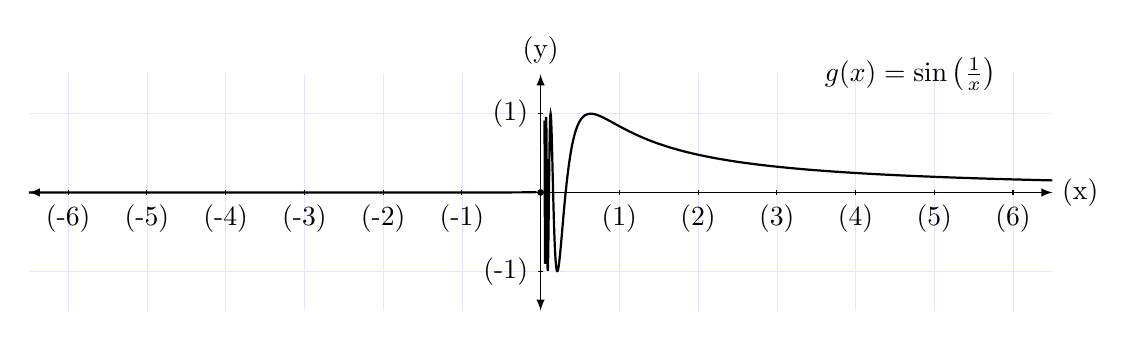
\begin{tikzpicture}[domain=-6.5:6.5,samples=4000,scale=1,>=latex]
\tikzset{bgrid/.style={help lines,color=blue!10,very thin}}
\draw[bgrid] (-6.5,-1.5) grid (6.5,1.5);
\draw[<->, color=black] (-6.5,0) -- (6.5,0) node[right] {(x)};
\draw[<->, color=black] (0,-1.5) -- (0,1.5) node[above] {(y)};
\foreach \x/\xtext in {-6,-5,-4,-3,-2,-1,1,2,3,4,5,6}
\draw (\x cm,1pt) -- (\x cm,-1pt) node[anchor=north] {(\xtext)};
\foreach \y/\ytext in {-1,1}
\draw (1pt,\y cm) -- (-1pt,\y cm) node[anchor=east] {(\ytext)} ;
\draw[thick,color=black,domain=-6.5:-0.05,samples=2000] plot (\x,{-1*sin(1/\x r)});
\draw[thick,color=black,domain=0.05:6.5,samples=2000] plot (\x,{sin(1/\x r)});
\filldraw (0,0) circle (1pt);
\draw (4.7,1.5) node {$g(x) = \sin \left(\frac{1}{x}\right)$};
\end{tikzpicture}
\end{center}

\end{document}